%==============================================================================
%== template for LATEX poster =================================================
%==============================================================================
%
%--A0 beamer slide-------------------------------------------------------------
\documentclass[final]{beamer}
\usepackage[orientation=portrait,size=a0,
            scale=1.25         % font scale factor
           ]{beamerposter}
      
\geometry{
  hmargin=2.5cm, % little modification of margins
}
%
\usepackage{tikz}
\usetikzlibrary{mindmap}
%
\usepackage[utf8]{inputenc}
\usepackage[T1]{fontenc}
\usepackage{babel}
\usepackage{graphicx}
\usepackage{amsmath}
\linespread{1.15}
%
%==The poster style============================================================
\usetheme{sharelatex}

%==Title, date and authors of the poster=======================================
\title
[JDEV 2017, 4ème édition des Journées nationales du DEVeloppement logiciel, Marseille, 4, 5, 6 et 7 juillet 2017.] % Conference
{ % Poster title
Développement de paquets Nix (nixpkgs)
}

\author{ % Authors
Bruno Bzeznik\inst{2},Laure Tavard\inst{2}, ... etc ... Philippe Beys (liste des auteurs)\inst{1}
}
\institute
[CNRS/UGA] % General University
{
\inst{1} Service Informatique, Laboratoire LIPHY, UMR5588, CNRS, Université Grenoble Alpes\\[0.3ex]
\inst{2} UMS GriCAD, CNRS, Université Grenoble Alpes\\[0.3ex]
}
\date{\today}

\begin{document}
%\begin{frame}[t]
\begin{frame}[fragile]
%==============================================================================
\begin{multicols}{3}
%==============================================================================
%==The poster content==========================================================
%==============================================================================
\section{Introduction et Historique}

Nix\cite{ref1} est un gestionnaire de paquets qui utilise un langage fonctionnel. Ce gestionnaire de paquets s'installe sur Linux, OS X et NixOS. Il est issu des travaux de recherche d'Eelco Dolstra\cite{ref2} publiés dans sa thèse\cite{ref3}  à la Technische Universiteit de Delft. La communauté des utilisateurs a poursuivi ses travaux et Nix est devenu   aujourd'hui tout un ecosystème.   
\begin{figure}
\centering

\includegraphics[width=0.49\columnwidth]{nixos-logo.png}
\caption{Logo Nix}
\end{figure}
\section{Pourquoi utiliser Nix}

Nix permet l'installation de paquets dans le répertoire des utilisateurs, des mises à jour réversibles. Il permet de faire cohabiter plusieurs versions de logiciels différentes.

\vspace{0.5cm}
Il est fiable: par une approche purement fonctionnelle Nix s'assure que l'installation ou la mise à niveau d'un paquet ne puisse pas casser d'autres paquets. En effet, Nix ne remplace pas les dépendances existantes avec des versions plus récentes (ce qui pourrait être à l'origine d'une nouvelle rupture de dépendance). Nix vous permet de revenir à des versions précédentes, et veille à ce qu'aucun paquet ne se trouve dans un état incohérent lors d'une mise à niveau.

\vspace{0.5cm}
Il est reproductible: Nix construit des lignées de paquets isolées les uns des autres. Cela garantit que les installations sont reproductibles et n'ont pas les dépendances non déclarées. Si un paquet fonctionne sur une machine, il sera également capable de fonctionner sur une autre.

\vspace{0.5cm}
Nix est idéal pour les développeurs: Nix rend simple la mise en place d' environnements pour vos projets, quels que soient les langages de programmation et des outils que vous utilisez.

\vspace{0.5cm}
Nix est multi-utilisateurs, multi version: Nix suppoprte la gestion des paquets multi-utilisateurs: plusieurs utilisateurs peuvent partager un magasin Nix commun (nix store) en toute sécurité, sans avoir besoin des privilèges root pour l'installation. Les utilisateurs peuvent installer et utiliser différentes versions d'un paquet.

\section{Installation}
Si vous êtes sur Linux ou Mac OS X, le plus simple est de lancer la commande suivante:

\begin{verbatim}
$ bash <(curl https://nixos.org/nix/install)    
\end{verbatim}

Pour supprimer Nix de votre machine, à tout moment, il suffit de faire:
\begin{verbatim}
$ rm -rf /nix
\end{verbatim}

\section{Premiers pas avec Nix}

\subsection{Liste des paquets installables}
\begin{verbatim}
$ nix-env -qa
2048-in-terminal-2015-01-15
2bwm-0.2
389-ds-base-1.3.5.15
.../...
\end{verbatim}

\subsection{Installer un paquet}

\begin{verbatim}
$ nix-env -i python
\end{verbatim}

\subsection{Mettre à jour les paquets}
\begin{verbatim}
$ nix-env -u
\end{verbatim}

\subsection{Voir les versions de gcc installées}
\begin{verbatim}
$ nix-env -qaf nixpkgs-version gcc
gcc-3.4.6
gcc-4.0.3
gcc-4.1.1
\end{verbatim}

\subsection{les profils}
Il manque des explications ici !

\begin{figure}
\centering
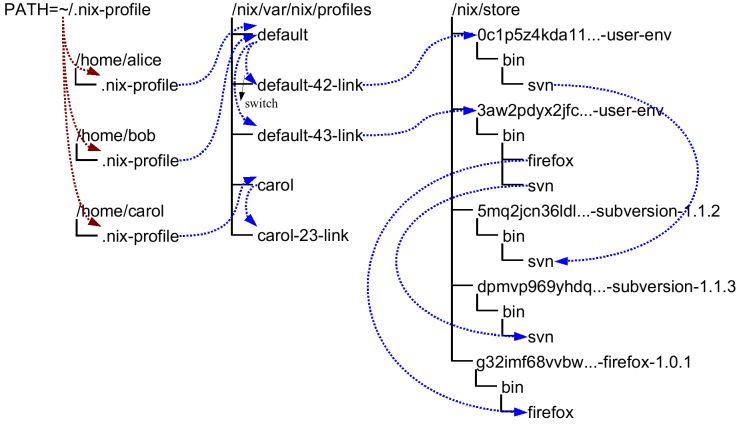
\includegraphics[width=0.99\columnwidth]{user-environments.png}
\caption{Environement utilisateur}
\end{figure}

\section{Gestion des environnements de développement}
Nix est extrêmement utile pour les développeurs car il installe l'environnement de construction des paquets. Étant donné une expression Nix qui décrit les dépendances de votre paquet, la commande nix-shell va construire ou télécharger les dépendances (si elles ne sont pas déjà dans votre magasin Nix) puis lancer un shell Bash dans lequel toutes les variables d'environnement nécessaires sont définies (compilateur et  différents chemins vers les ressources nécessaires).

\section{Développer son premier paquet nix}

\subsection{Installer le répertoire de développement nixpkgs}

\begin{verbatim}
$ git clone git://github.com/NixOS/nixpkgs.git 
$ cd nixpkgs
\end{verbatim}

\subsection{Ajouter un répertoire contenant la dérivation à rajouter}
Si vous développez la lilbrairie  ''malib''

\begin{verbatim}
$ mkdir pkgs/development/libraries/malib
\end{verbatim}

Pour construire le paquet correspondant, vous allez devoir écrire une dérivation. Une dérivation est une fonction (tout est fonction dans Nix). 

Pour un environnement standard, avec une construction du type: configure, make, make install, vous pouvez utiliser la fonction stdenv.mkDerivation fournie par Nix, ce qui va se traduire par:

\begin{verbatim}
stdenv.mkDerivation {
  name = "libfoo-1.2.3";
  src = fetchurl {
    url = http://example.org/libfoo-1.2.3.tar.gz;
    sha256 = "0x2g1jqygyr5wiwg4ma1nd7w4ydpy82z9gkcv8vh2v8dn3y58v5m";
  };
}
\end{verbatim}

Pour construire le paquet, il suffit de lancer la commande:

\begin{verbatim}
$ nix-build -A malib
\end{verbatim}

et c'est tout.

\section{Exemple de passage à l'échelle: du mésocentre au centre national}
Donner un exemple d'application packagée qui tourne sur Grenoble et sur un centre national, en montrant que le passage à l'échelle est automatique.











%==============================================================================
%==End of content==============================================================
%==============================================================================

%--References------------------------------------------------------------------

\subsection{Références}

\begin{thebibliography}{99}

\bibitem{ref1} \url{http://nixos.org/nix/}

\bibitem{ref2} \url{https://nixos.org/~eelco/}

\bibitem{ref3} \url{https://nixos.org/~eelco/pubs/phd-thesis.pdf}


\end{thebibliography}
%--End of references-----------------------------------------------------------

\end{multicols}

%==============================================================================
\end{frame}
\end{document}
